\chapter{Design and Implementation}
%You are free to write up any additional material that will appear in the final
%report, for example a section or chapter describing a significant component of
%the design/implementation that you have already completed.  Avoid any
%additional material that is not re-usable in the final report.

\section{Mathematical model}

We shall now introduce the new metric that can be seen as a generalisation of
the Graphlet Frequencies described above. This metric, which we shall call the
Graphlet Cluster Vector (for reasons that will soon become obvious), is
a key element of this project. As this is a novel metric, we would like to
explore its properties and compare it to the Graphlet Frequency Vector and
Graphlet Degree Distribution described above. 

For a particular graph G and node n in G, we denote by \( S_n \) the
set of neighbouring nodes of n and by \( S_n^i\) the number of graphlets of
type i in \( S_n \). Now, we consider the \emph{Graphlet Cluster Vector} to be:

$$ GCV(n) = \left(F_n^1, F_n^2, ... F_n^{29}\right)$$

where

\begin{equation}
 F_n^i = \frac{S_n^i}{\sum_{i=1}^{n}S_n^i}
\end{equation}
 
The new Graphlet Cluster Vector (GCV) metric is therefore
generalising the GDV so that it includes information from the cluster of
neighbouring nodes. 

\subsection{Relative Cluster Frequency Distance}

Similarly to how the Relative Graphlet Frequency Distance is calculated, we
will now define a similar measure for the distance measure for the new GCV
signature. If we consider two nodes p and q in graph G and we denote \(F_p^i\)
and \(F_q^i)\) to be the frequency of the i-th graphlet in nodes p and q, then
we compute the \emph{Relative Cluster Frequency Distance} (RCFD) as follows:

\begin{equation}
 RCFD(p,q) = \sum_{i=1}^{n}| F_p^i - F_q^i |
\end{equation}

\section{Implementation of the Graphlet Cluster Vector}

After the first stage of the project has been done, which was concerned with
the mathematical model behind the Graphlet Cluster Vector, we started
implementing the model in the C++ programming language. The two main reasons for
implementing the algorithm in C++ were:
\begin{enumerate}
 \item Dr. Przulj's research group already had a C++ function that was able to
count the number of graphlets in a given graph. We were therefore able to
leverage that code.
 \item As, C++ is a compiled language that does not run in a virtual
environment, it is computationally-speaking really fast. Since our algorithm
was meant to execute very intensive calculations on large biological networks,
it was therefore a good decision to use C++. 
\end{enumerate}

The C++ file that I was given from Przulj's group, called ncount.cpp, was used
to count both the number of graphlets in a graph and also the number of
automorphism orbits that nodes would touch. I also received three types of
networks to test my algorithm on:
\begin{enumerate}
  \item Protein-protein interaction network: Such networks describe the physical
contacts established between two or more proteins as a result of biochemical
processes or electrostatic forces. In this network, nodes would correspond to
proteins and would get connected by an edge if there is a direct interaction
between the underlying proteins. 
  \item Metabolic network:  These networks describe the complete set of
metabolic and physical processes that determine the physiological and
biochemical properties of a cell. As such, these networks are composed of
metabolic pathways as well as regulatory interactions that guide the chemical
reactions taking place.
  \item Trade network: This network describes the amount of economic trade
that has been taking place in 2010 between major countries around the world.
For each pair of countries, a number was given describing the trade volume that
took place between them in 2010. This network would be ideally modeled using a
weighted network. However, since our algorithm works only on unweighted
networks, we had to trim down the edges between two countries that traded less
than a certain volume of goods. 
\end{enumerate}

A third and last script that I was given was used to convert the given networks
to a file format called LEDA, that is easy to be read and processed by the
graphlet counting function.

\subsection{Node-based Graphlet Cluster Vector}

I started writing the code by first modifying the graphlet counting function
(from ncount.cpp) and removed the unnecessary code that was dealing with
automorphism orbits. Afterwards, I realised that the function was still hard to
work with, for it was way too long and seemed to resemble a 'God-function' that
was responsible for everything: reading from the input file, parsing it,
building an efficient data structure to store the input in, counting the
graphlets and writing to the output file. I therefore decided to split it up
into modules according to their responsibility, concepts I learned from the
Software Engineering course in the second year. 

Afterwards, I started writing the code that would iterate over each node in the
input graph and extract the neighbouring subgraph (i.e. the graph containing
all the neighbours of a particular node plus the edges between them.). It is
worth mentioning that, for a given node $n$, the neighbouring subgraph of $n$
does not contain $n$ itself, nor any of the edges between $n$ and its
neighbours. 

This part of the code took a while to implement mainly because I
had to deeply understand how the data structure what was used to store the
graph worked. The programmers who implemented the initial graphlet-counting
function were using a specially-optimised data structure that was storing the
network both in an adjacency matrix and in an adjacency list at the same time.
This turned out to be a good idea, because using both the list and the matrix
forms allowed for many operations to be executed in O(1) time:
\begin{itemize}
 \item The adjacency matrix allowed one to check whether two arbitrary nodes
are connected in O(1) time.
 \item The adjacency list allowed one to get the list of all the neighbours of
a node in O(1) time. This was especially useful for my extended function, where
I needed to extract the neighbourhood of a node in order to count the number of
graphlets in it. 
\end{itemize}

After I understood the underlying concepts behind the optimised data structure, I
implemented the neighbourhood extraction part of the algorithm and unit tested
it using some manually crafted network examples of up to 20 nodes. Once the
neighbourhood extraction phase was complete, I passed the neighbourhood to the
graphlet counting function (ncount) and I got a signature made of 29
frequencies, one for each graphlet type. From here, it was simple to repeat the
operation over all the nodes in the input network.

\subsection{Parallelisation}

Soon after I started testing the newly-written algorithm on the large
biological networks, I realised that the algorithm was taking hours to finish
calculating the GCV for every node in the network. Therefore, I have decided to
paralellise the code across multiple cores by forking different threads. I have
decided to do this as an initial improvement, and if there was need for even
more parallel processing, I would later on extend it to run on a cluster of
computers.

\hilight {insert chunking diagram here}

The most effective way to parallelise was to split the node set into N chunks
and then have each thread compute GCV signatures for all the nodes from the
corresponding chunk. The advantae of forking different threads is that they
have access to the same shared memory, so all of them could access the same
input data easily. At the end, I made it work so that the desired number of
threads could be passed as a command line argument, and changed the Makefile
accordingly.

Each thread would write the output to its own file, which had the thread id at
the end of its name. This way, the master thread would wait until all its
children have finished processing and then it would compile the output files
from each child thread into a single file. 

%See table \hilight{table citation} for a reference of the size of the
%networks. 


\hilight{Include a table that shows the network size(nodes and edges) + the
time improvements obtained from paralellising across multiple cores}

\subsection{Average Network GCV}

Once the GCV signature of every single node in the input network was
computed, I wrote a different C++ program that would take these signatures and
compute an average GCV signature for the whole network. This allowed me to
perform comparisons between various network types, both real networks as well
as random networks.


\begin{figure}[h]
  \centering
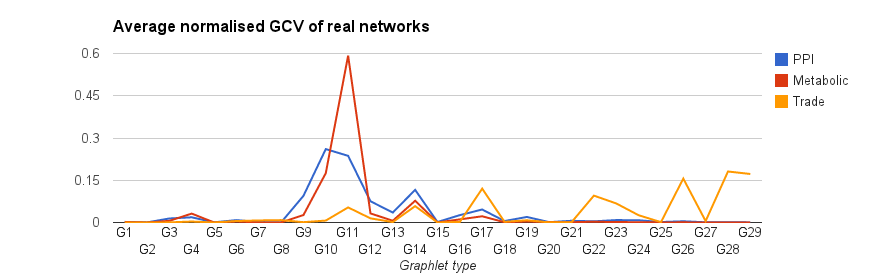
\includegraphics[scale=0.5]{charts/1-avg-norm-ppi-all.png}
\caption{Comparison of the graphlet degree vectors for three different
real networks: Protein-protein interaction network, Metabolic network and 
a 2010 Trade network between countries}
\label{fig:avg_gdv_real}
\end{figure}

What we observe from figure \ref{fig:avg_gdv_real} is that there are slight
differences between the GCV of the three networks analysed. More precisely,
Graphlets $ G_{11} $ and $ G_{10} $ seem to discriminate well between them,
with the Metabolic network having the highest number of type $ G_{11}$ graphlets
while the trade network having the least. Moreover, the trade network also seems
to have considerably more graphlets of type $ G_{22}, G_{26} $ and $ G_{28}$. 


\subsection{Random Networks}

After we performed a few comparisons of the average GCV of real networks, our
next step was to experiment with the following random network models:
 \begin{enumerate}
    \item Erdos-Renyi\cite{erdHos1959random}
    \item Erdos-Renyi (arbitrary degree distribution)
    \item Geometric networks\cite{penrose2003random}
    \item Barabasi-Albert (preferential attachement)\cite{barabasi1999emergence}
    \item Stickiness index-based\cite{prvzulj2006modelling}
  \end{enumerate}

We have performed one initial experiment on the Human PPI network, using both
the real network and the random models mentioned above(see fig.
\ref{fig:avg_gdv_ppi_random}). We have not had
enough time to calculate the GDV agreements between these networks, but once
that is done we would be able to tell how well the random models fit the data
and which random model fits the real network best. 

\begin{figure}[h]
  \centering
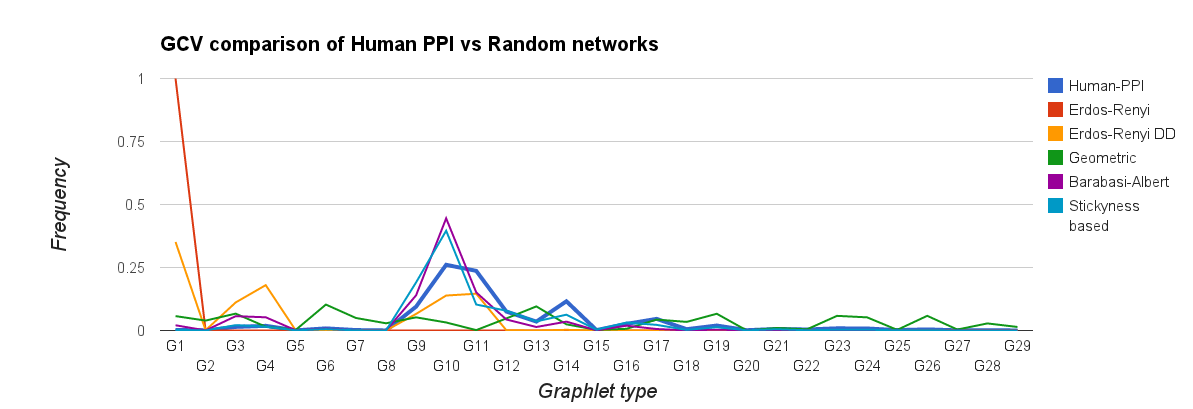
\includegraphics[scale=0.4]{charts/2-avg-norm-ppi-vs-random.png}
\caption{Comparison of the graphlet degree vectors between Human PPI network
and random models: Erdos-Renyi, Erdos-Renyi with the Degree Distribution of the
Human PPI network, Geometric, Barabasi-Albert Preferential Attachment,
Stickiness-based}
\label{fig:avg_gdv_ppi_random}
\end{figure}

  
\section{Upcoming tasks}

The next task that I am looking into is to compute the Graphlet Frequency
Agreement between random networks and real networks. This will allow us to find
out which models best fit the data. Afterwards, I will generate more instances
of each type of random networks in order to find out what is the standard
deviation of the frequencies in the GCV. This would allow us to establish how
robust the new GCV signature is to noise.